%\chapter{Tätigkeitsbericht}
\label{chap:Taetigkeitsbericht}


\section{Chronologischer Tätigkeitsabriss}
\label{sec:Chronologischer_Taetigkeitsabriss}
\begin{figure}[htb]
  \centering  
  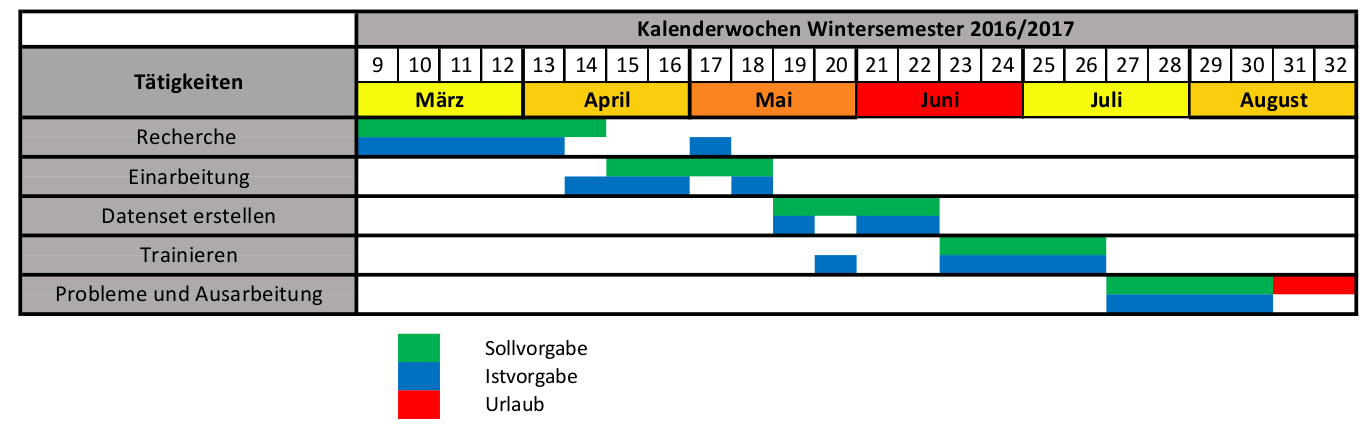
\includegraphics[scale=0.35]{img/GANTT-Diagramm.png}
  \caption{GANTT-Diagramm \cite{Gantt}}
  \label{fig:GANTT-Diagramm}
\end{figure}


\section{Internetrecherche}
\label{sec:Recherche}
Zu Beginn des Praktikums hatte ich wenige Vorkenntnisse in Action-Recognition und mit welchen Künstlichen Neuronalen Netzen man dies Umsetzen kann. Deshalb habe ich eine recht lange Recherchephase eingeplant, um mich mit dem Grundlagen des Thema ausführlich zu befassen. Es stellte sich heraus, dass es verschiedene Ansätze zur Actions-Recognition gibt:

\begin{itemize}
\item LSTM (Long- Short- Time Memory)
\item 3D Convolutional Networks
\item Two Stream 3D Convolutional Networks
\end{itemize}

Es gab viele Informationen und etliche Papers zu diesem Thema. Im Paper Quo Vadis, Action Recognition? A New Model and the Kinetics Dataset \cite{DeepMind/i3d} von GoogleDeepMind. Sie stellten verschiedene Ansätze nebeneinander und verglich welche Möglichkeiten sich als effektiv herausstellten. Das beste Netz dieses Papers war das Two-Stream 3D-Convolutional Netz, welches die besten Ergebnisse lieferte. Von Deep Mind wurde das Framework für dises Netz über Github frei zugänglich gemacht.

\section{Einarbeiten in vorhandene Frameworks}
\label{sec:Einarbeiten}
Die Einarbeitung gestaltete sich schwieriger als zuerst angenommen, da keine Funktionen zum Trainieren und Testen mitgeliefert wurden. Als Programmiersprache wurde Python benutzt und wie für DeepMind klassich wurde, als Front-End Sonnet, welches on top on Tensorflow aufbaut. Desweiteren habe ich ein Opensource Projekt der University of Science and Technology of China gefunden, welche ein Github Reposetorie zur Verfügung stellten, welches es ermöglichte dieses Netz zu trainieren und zu testen und von mir für unseren Anwendungsfall angepasst werden konnte.

\begin{figure}[htb]
  \centering  
  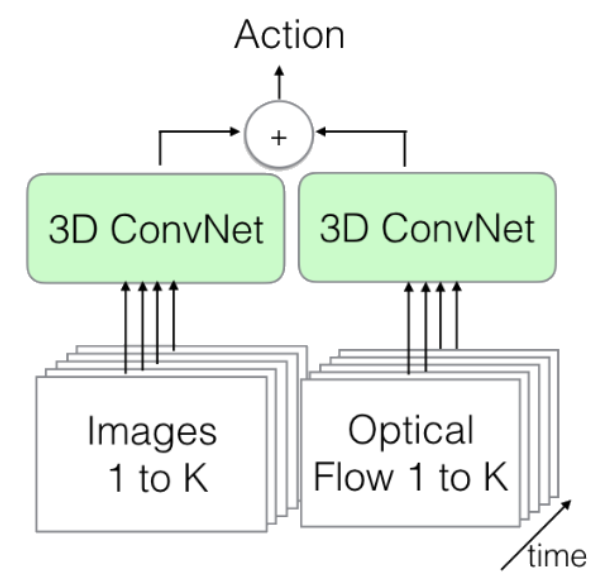
\includegraphics[scale=0.5]{img/Two-Stream.png}
  \caption{Two-Stream 3D-ConvNet  \cite{DBLP:journals/corr/CarreiraZ17}}
  \label{fig:Two-Stream 3D-ConvNet}
\end{figure}

Was heißt Two-Stream 3D-ConvNet?

Es handelt sich um zwei 3D-ConvNets. Eins für die Verarbeitung von RGB-Videos und eins für die Verarbeitung von Optical Flow Videos mit einer anschließenden Zusammenführung der Ergebnisse. Damit hat man stabilere Ergebnisse als nur einzelne Streams.

\newpage

\section{Optical Flow}
\label{sec:OpticalFlow}
Optical Flow ist die Bewegung von einzelnen Pixeln in X und Y Achse von zwei aufeinander folgende Frames eines Videos. Dieser Optical Flow wurde anfangs beiseite gelassen, um einen einfacheren Einstieg zu ermöglichen. Jedoch, zu einem späteren Zeitpunkt mit integriert. Um diesen Optical Flow zu extrahieren wurde von der Bibliothek Open-CV2 der Dense Optical Flow Alorythmus verwendet. Ich habe auch ein Künstliches Neuronales Netz das FlowNet2.0 \cite{FlowNet2.0} versucht für die Generierung des Optical Flow Images zu verwenden. Dies lieferte bessere Ergebnisse, dennoch war die Umsetzung zu Rechenaufwändig und somit für spätere Echtzeitanwendungen nicht brauchbar.

\begin{figure}[!htb]
  \centering
  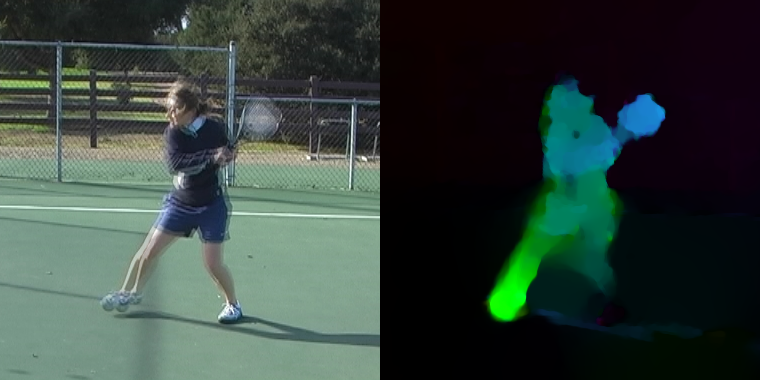
\includegraphics[scale=0.3]{img/tennis.png}
  \caption{Optical Flow   \cite{Bro11a}}
  \label{fig:Optical FLow}
\end{figure}

\section{Erstellen von Trainings- und Testdaten (Datenset)}
\label{sec:Datenset}
Ursprünglich wurde angedacht die Trainingsdaten mit der Microsoft Hololens zu erstellen. Da die Aktionserkennung auch für das Projekt mit der Hololens gedacht war. Dennoch stellte sich nach einigen Versuchen heraus, dass der Sichtwinkel der Hololence äusserst ungünstig ist und die Hände nur bei ausgestreckten Armen zu sehen sind. Dies ist aber keine natürliche Haltung. Um trotzdem ein Datenset zusammen zustellen wurde eine GoPro mit Kopfgurt benutzt. Welches mir es ermöglichte die Arbeiten unter normalen umständen aufzunehmen. Es war wichtig, an verschiedenen Orten und mit verschiedenen Personen diese Videos aufzunehmen, um gute aber gewollte Varianz in den Trainingsdatenset zu bekommen. 80\% der Videos wurden im FZI aufgenommen und 20\% der Videos wurden in der Uni-Clinc Heidelberg aufgenommen. Natürlich wäre es am Besten gewesen Videos aus realen Verbandswechsel mit Patienten zu haben, dies war aber aus rechtlichen Gründen (Datenschutz) noch nicht möglich.

 Es wurden ein Datenset zu folgenden Klassen erstellt:
\begin{itemize}
\item Gloves on (Anziehen von Handschuhen)
\item Clean (Putzen/Desinfizieren der Ablage)
\item unpacking (Auspacken der Verschlossenen Materialen wie Plaster und Verband)
\item Gloves off (Ausziehen von Handschuhen)
\item Disinfekt (Desinfiziernen der Hände)
\item Other (Verschiedene Actionen aus der Egoperspektive)
\end{itemize}


\section{Trainieren eines 3D-ConvNets}
\label{sec:Trainieren}
Um ein Netzwerk dieser Größe zu trainieren werden große Rechenleistungen benötigt. Deshalb wurde das Netz von Googles Deepmind auf das ImageNet Datenset vor trainiert. Dies brauchte auf 11 Tesla GPUS mehrer Wochen Training. Dieses Netz kann dann fine-getuned werden, also auf unsere Anwendungen angepasst werden. Das Finetunen funktioniert wie folgt: man schneidet die letzten Fully Connectet Layer ab und trainiert diese dann auf seine eigenen Daten neu. Somit ist es möglich, ein Netz in kurzer Zeit mit wenig Daten zu trainieren und zusätzlich noch gute Ergebnisse zu erhalten.


Das Training mit den RGB-Videos funktionierte gut. Und ergab nach den ersten Versuchen gute Ergebnisse. Das Ganze wurde dann mit Optical Flow wiederholt, somit hat man zwei Netze die einmal RGB Images und Optical Flow Images Verarbeiten können. Diese Ergebnisse werden anschließen zu einer Aussage zusammengefasst. Diese kann man dann mit einem Evaluierungstest auswerten.
